%%%%%%%%%%%%%%%%%%%%%%%%%%%%%%%%%%%%%%%%%
% University Assignment Title Page 
% LaTeX Template
% Version 1.0 (27/12/12)
%
% This template has been downloaded from:
% http://www.LaTeXTemplates.com
%
% Original author:
% WikiBooks (http://en.wikibooks.org/wiki/LaTeX/Title_Creation)
%
% License:
% CC BY-NC-SA 3.0 (http://creativecommons.org/licenses/by-nc-sa/3.0/)
% 
% Instructions for using this template:
% This title page is capable of being compiled as is. This is not useful for 
% including it in another document. To do this, you have two options: 
%
% 1) Copy/paste everything between \begin{document} and \end{document} 
% starting at \begin{titlepage} and paste this into another LaTeX file where you 
% want your title page.
% OR
% 2) Remove everything outside the \begin{titlepage} and \end{titlepage} and 
% move this file to the same directory as the LaTeX file you wish to add it to. 
% Then add \input{./title_page_1.tex} to your LaTeX file where you want your
% title page.
%
%%%%%%%%%%%%%%%%%%%%%%%%%%%%%%%%%%%%%%%%%
%\title{Title page with logo}
%----------------------------------------------------------------------------------------
% PACKAGES AND OTHER DOCUMENT CONFIGURATIONS
%----------------------------------------------------------------------------------------

\documentclass[paper=a4, fontsize=11pt]{scrartcl}
\usepackage[english]{babel}
\usepackage[utf8x]{inputenc}
\usepackage{mathtools}
\usepackage{graphicx}
\usepackage[colorinlistoftodos]{todonotes}

\begin{document}

\begin{titlepage}

\newcommand{\HRule}{\rule{\linewidth}{0.5mm}} % Defines a new command for the horizontal lines, change thickness here

\center % Center everything on the page
 
%----------------------------------------------------------------------------------------
% HEADING SECTIONS
%----------------------------------------------------------------------------------------

\textsc{\LARGE EURECOM}\\[1.5cm] % Name of your university/college
%\textsc{\Large Major Heading}\\[0.5cm] % Major heading such as course name
%\textsc{\large Minor Heading}\\[0.5cm] % Minor heading such as course title

%----------------------------------------------------------------------------------------
% TITLE SECTION
%----------------------------------------------------------------------------------------

\HRule \\[0.4cm]
{ \huge \bfseries Music Recommendation when Exploring a City}\\[0.4cm] % Title of your document
\HRule \\[1.5cm]
 
%----------------------------------------------------------------------------------------
% AUTHOR SECTION
%----------------------------------------------------------------------------------------

\begin{minipage}{0.4\textwidth}
\begin{flushleft} \large
\emph{Authors:}\\
Lorenzo \textsc{Canale} % Your name
\newline
Fabio \textsc{Ellena} % Your name
\end{flushleft}
\end{minipage}
~
\begin{minipage}{0.4\textwidth}
\begin{flushright} \large
\emph{Supervisor:} \\
Pasquale \textsc{Lisena} % Supervisor's Name
\end{flushright}
\end{minipage}\\[2cm]

% If you don't want a supervisor, uncomment the two lines below and remove the section above
%\Large \emph{Author:}\\
%John \textsc{Smith}\\[3cm] % Your name

%----------------------------------------------------------------------------------------
% DATE SECTION
%----------------------------------------------------------------------------------------

%{\large \today}\\[2cm] % Date, change the \today to a set date if you want to be precise

%----------------------------------------------------------------------------------------
% LOGO SECTION
%----------------------------------------------------------------------------------------

%
\includegraphics{logo.png}\\[1cm] % Include a department/university logo - this will require the graphicx package
 
%----------------------------------------------------------------------------------------

\vfill % Fill the rest of the page with whitespace

\end{titlepage}
\tableofcontents
\newpage
\begin{abstract}
Common music recommender systems do not take into account the position of the customer. This piece discusses how it is possible to link a song with a POI using the semantic web.
\end{abstract}

\section{Introduction}
Linkng POIs and songs is a big challenge, in fact they are part of two completely separated concepts that cannot be easily linked also by a person it would be difficult to state some criteria that can link a song with a place. We present an approach that attempts to leverage this problem by using the semantic relations exposed by DBpedia.
\subsection{Motivation and context}

\subsection{Research problems}

\subsection{Contributions}

\subsection{Report structure}
The report is divided into four sections, one for each part of the project. The first two parts are about linking external datasets to Dbpedia, this is also known as enrichment and it consists of linking in the correct way two entities of different datasets
\section{Interlinking and enriching POIs}

\subsection{Problem description}
Finding relations inside DBpedia is a known problem which has been resolved in the past. So we could simply look for POIs and Artists in Dbpedia and then link them using known algorithms.
Unfortunately DBpedia is not perfect: it is true that it contains POIs and Artists, but these entities are not cleanly defined, they usually contains dirty data that can tremendously affect our performances.
POIs and Artists can be found in highly specialized datasets, but unfortunately they do not contain links to eachother, and even worse they are not linked to DBpedia. This means that by using these databases alone we cannot find relations.
What is done in this cases is to link highly specialized datasets to DBpedia, in this way we can exploit the advantages of both worlds: highly specialized datasets give us confidence and trust in our main entities (POIs and Artists), while DBpedia allow us to find relations between them thanks to its generality.
The following two sections will explain in a detailed way the whole process of connecting these highly specialized datasets to DBpedia.

\subsection{Datasets: 3cixty, DBpedia, Wikidata}
\subsubsection{3cixty}
3cixty is a semantic dataset that contains aggregated informations of POIs and events. The dataset is the result of an aggregation process that join the POI informations from different datasets e.g. Facebook, Foursquare, Yelp \dots
In this project 3cixty is used as a trusted source of POIs for Nice.
POIs have many informations, such as the category, the address, comments from users, and coordinates. In order to get all the POIs in Nice, we simply used the POIs endpoint selecting the Nice city.
\subsubsection{DBpedia}
DBpedia is a project that aims at connecting the semantic world. We used it to get the POIs in Nice.
In order to get the POIs from DBpedia, it is necessary to perform SPARQL queries against the SPARQL endpoint. POIs are retrieved using two different sparql queries that target different kind of resources:
\begin{enumerate}
\item We perform a query that looks for all Geoentities that are in the area of nice. An entity is in the area of Nice if its coordinates are in a custom box that contains all the area of Nice.
Unfortunately there are many POIs that are without coordinates,so they are not selected with this query.
\item We perform some queries that get in a recursive way all entities that have as a parent the category of nice or nice and that are related to a place. The relation to a place is a list of classes that is done by hand and could be subjected to refinements.
\end{enumerate}
\subsubsection{Wikidata}
Wikidata is a project that aims at connecting the semantic world. We used it to get the POIs in Nice. Respect to DBpedia, Wikidata has a well defined ontology that is strictly enforced. This means that it is easier to select what we want. Moreover, most of POIs in wikidata have coordinates, so we can get them with a single query. Since wikidata supports complex geo-based queries, we made a query that looked for all POIs in a range of 25 Kilometers from the center of Nice.
\subsection{Entity Linking process}
Now that we have locally all our entities, we can link them. Having the entities locally is crucial, in fact it allows us to make way more complex operations respect to those that can be done with SPARQL queries.
\subsubsection{Properties}
The first phase is to actually get the interesting properties of the entities. Regarding those that come from DBpedia, we take use only the labels. We do not use coordinates because not all entities have them and we do not want to bias our algorithm using DBpedia coordinates, which is known that are not very accurate. Regarding the labels, we take all labels from all entities, in this way we are going to do a multilingual match because we know that sometimes this can make the difference.
Respect to Dbpedia, 3cixty entities have very accurate coordinates, and few labels. For this phase we do not need the coordinates, while regarding the labels, we keep the first one.
\subsubsection{Transformations}
At this point of the pipeline, we have labels that are encoded in unicode utf-8. Common similarity metrics accepts only plain ASCII strings as input, so we need to convert them into ASCII. Since utf-8 can represent way more characters than ASCII, we need to strip non ASCII characters from our labels. This is done in an intelligent way using the python library 'unidecode', that is able to convert from unicode to ASCII deleting only few characters. For example, an accented letter like 'è' can't be represented in ASCII. Most of the libraries delete all incompatible characters, while 'unidecode', when possible, converts it to the nearest ASCII character, in this case 'è' is converted to 'e'. In this way we can retain most of the original information after this conversion process.
The second step is probably the most important, and is the normalization of names. Some similarity metrics are extremely sensitive to noise. For example, when we use simple levenstein distance between ('aeroport','aeroport nice') is 5, while the distance ('aeroport','port') is 4. This is enough to raise some concerns: the simple addition of the city name can turn a perfect match into a mediocre one. In order to fix this problem we add the city name to all the labels where this is not present.
The third step is to strip all not alphabetical characters and to convert to lowercase all strings, this offcourse gives us cleaner strings to compare.

\subsubsection{Similarity measures and matching algorithm}
Now that strings are clean, we can proceed to the matching. A first problem rises: we want to match a 3cixty poi to a dbpedia poi, or we want to match a dbpedia poi to a 3cixty poi? In the first case we are sure that each 3cixty poi will be matched to a single dbpedia poi, but there is the risk that multiple 3cixty poi are matched to the same DBpedia poi. Alternatively, we match are sure that each DBpedia poi is matched to at most a 3cixty poi, but there is the risk that two DBpedia poi are matched to the same 3cixty poi.
Regarding DBpedia, we are sure that POIs are univoque, while we know that for the same POI, in 3cixty there are multiple ones.
Since at the end we will be using 3cixty coordinates, we opt for the first choice: if a DBpedia poi will be matched to multiple 3cixty pois, than we will follow an heuristic to choose the best match.
Regarding similarity metrics among strings, there are multiple ones, but most of them are based on levenstein distance.
Since each distance has its privileges and defects, we use multiple similarity measures, taken from the 'fuzzy wuzzy' python library.
For each 3cixty poi get the label and calculate the different similarity metric against all labels of all DBpedia POIs.



\subsubsection{Aggregations}
The aggregation algorithm can be described as follow:
\begin{enumerate}
\item For each similarity metric, take the three best matches and for them average the score of all similarity measures
\item The final match is the POI corresponding with the string with the highest score
\end{enumerate}
Why we don't simply take the average, or the minimum, or the maximum?
The reasoning behind this is that by taking the average we are flattening all the scores, and there is the risk that the string with the highest similarity is a string that is mediocre in all the different metrics. If a string is mediocre in all comparisons, then we do not trust it. Instead, with our methodology we are keeping only those matches that excel in some similarity metric, and then we take the one that performs better on average. We think that in this way we can filter out all those matches with average strings that matches almost anything.

\subsubsection{Filtering}
Now that the matching is done, we need to filter our results.
The first filter to do is to eliminate all those matches that match with Nice, but that have a label different from Nice. This usually happens because we added Nice to all strings. That addition was helpful, and it also created a safe default that now can be easily filtered.
Most of these match are acronym that match with Nice e.g. 'ATP Nice' matches with Nice because half of the string is Nice and is artificial, because we added it.

At this point we filter out all matches with a score below a given threshold.

Then, we have probably multiple 3cixty POIs connected to a single DBpedia POI.
In order to choose the most representative 3cixty POI, from whom we will take the coordinates, we have few possibilities:
\begin{enumerate}
\item K-medoids: We can actually cluster our points and look at the rapresentant of the biggest cluster 
\item Pick the POI which is nearest to the center
\item Pick the POI which is nearest to the DBpedia POI, if coordinates are available
\item Pick the POI which is nearest to the position found on OpenStreetMap
\item Link our data to GeoNames, a dataset of POIs
\end{enumerate}
The first method might be the best one, but it requires several precautions.
The second method is baiased towords pois in the center.
The third method can work only with POIs with coordinates, and gives good results if DBpedia coordinates are good, but we already know that this is not true.
The fourth method might be the best one, but we need to exit from the semantic world and hope that the API gives a good result, here the problem is that we have no control over the API.
The fourth method can work, but we would need to design another linking process.

For simplicity and reliability, we decided to use both OpenStreetMap API and Google Map API, in this way we have a much bigger confidence.

We make a request with the DBpedia label to the API, and we keep the POI which is nearest to one of them, in this case the minimum distance wins. If the distance is greater than a chosen threshold (500 meters), then the match is filtered out. 

\subsection{Evaluation (Google Map / OpenStreetMap)}
The evaluation part is done using both the Google Map and OpenStreetMap. We calculated the Medium Square Error of the POIS to the positions recovered with the APIs, the error distance is the haversine distance.
\section{Interlinking and enriching Artists}
\subsection{Problem description}
\subsection{Datasets: DOREMUS, DBpedia, Wikidata}
\subsection{Entity Linking process (+ ElasticSearch)}
\subsubsection{Properties}
\subsubsection{Transformations}
\subsubsection{Similarity measures}
\subsubsection{Aggregations}
\subsubsection{Filtering}
\subsection{Evaluation}
\section{Path finder}
\subsection{Problem description}
\subsection{Related work (relfinder)}
\subsection{Proposed approach and best path selection algorithm}
\section{REST API}
The paths between a POI and the linked artists are exposed by a REST API that runs on Flask. Their extensible framework allows to develop several components requiring minimum boilerplate.
The main endpoint is the one that exposes the tracks and the paths related to a specific geoposition.
The whole process can be summarized in:
\begin{enumerate}
\item Take user position
\item Calculate nearest POIs and assign weights, from these create a univoque playlist name.
\item Select the tracks for each artist linked with the poi.
\item Select for each artist a compatible number of tracks to put in the playlist.
\item Create a playlist if it does not exist and add previously selected tracks.
\item Attach to each track the path between the poi and the track's artist.
\item Return the playlist ID and the track-path mappings as a JSON.
\end{enumerate}
\subsection{Spotify API usage}
Spotify provides a public API that allows to perform all the operations that can be done using the Spotify application. These comprend artist and tracks search, CRUD operations on user playlists and the listening of the tracks' preview.
\subsubsection{Authentication}
Since the end user listen to a spotify loaded dynamically by the application, there is no need for a client authentication. This is perfect because it allows to any user to use our application. Regarding the server, At startup it is performed a token based authentication, where the server get possess of a private token used to perform all CRUD operations on the playlist catalogue.
\subsubsection{Playlist}
A playlist can be dynamically created. At creation time, it is required to give a name to the playlist, and the whole playlist object, containing the univoque playlist ID is returned. Later it is possible to access to the playlist either using the playlist ID or using the playlist name. The playlist name is univoque inside the application by construction, while the playlist ID is univoque for all Spotify playlists.
\subsubsection{Artist}
An artist can be searched by name, this part is the most critical one because Spotify does not provide any automatic artist matching using the api. This means that specifying the full name of the artist is essential for the success of this operation.
This is done by using the Doremus person label property, which consists of name and surname of the artist. It is interesting to note that from this point of view DBpedia is not reliable because the person label can contains adjectives used for the disambiguation of this one, such as 'Composer'. If this adjectives are passed to the Spotify search endpoint, no artist is returned.
When a request is done, Spotify returns a list of matching artists. Each artist object contains different informations, among them the most useful are the genres and the popularity. 
In order to limit outliers, not only we select the most popular artist, but we check that it has at least 10 popular songs, where popular songs are special songs selected by spotify. The popularity metric algorithm is not public, but it is based on the playcounts and the recentness of the track.
Here we use the popularity as a criteria to select the correct artist, in fact we take always the most popular. The use of the genre specification would be interesting for an ulterior enhancement.
\subsubsection{Tracks}
Among all properties that caracterize a track, we only need the ID and the name.

\subsection{Playlist Endpoint}
\subsubsection{Nearest POIs selection algorithm}
In order to match a position with a list of POIs, the following algorithm is followed:
\begin{enumerate}
\item Calculate distance from the each POI to the user position. Since we are using coordinates, the distance is calculated using the haversine distance, which is very accurate and fast.
\item Add to the list the nearest POI, regardless of the distance.
\item Add the remaining two nearest POIs if their distance is inferior of 1 km.
\item For each element in the list, add 10 meters to the distance and then take the log2. By adding 10 meters we are adding a bias to all our distances, in this way positions too near to us are not over-weighted respect far distances. Then, the log2 squashes distances until 1 km to a restricted range of values.
\item Calculate repartition weights using the following equation:
$$w_i = \Bigg \lfloor 10 \dfrac{\dfrac{1}{\log_2 (d_i + 10)}}{\sum \dfrac{1}{\log_2 (d_i + 10)} } \Bigg \rceil$$
In this way we obtain normalized weights from 0 to 10 that are inversely proportional to the log base 2 of the distance. 
\end{enumerate}
At this point we have a direct mapping between POIs weights and a position
\subsection{Artist' tracks selection algorithm}
For each artist there is a direct mapping with its tracks.
The problem is: given a playlist name, find the correct tracks.
The playlist name encodes the weights of each poi, and each weight express exactly the number of tracks that must be chosen for the POI associated.
Since each POI is linked to different artists, we need a way to select songs from them in a balanced way.
What we do is to cycle between all the artists to take each time the most important song that is not already present in the playlist. In this way we obtain different songs from different artists, and since the artist and songs are static, the tracks in the playlist will be always the same. In the future we think to add randomicity to the whole selection process.

\subsection{Response generation}
\begin{enumerate}
\item Generate playlist name as described before
\item Select tracks as described before
\item Create a playlist if it does not exist and add previously selected tracks.
\item Attach to each track the path between the poi and the track's artist.
\item Return the playlist ID and the track-path mappings as a JSON.
\end{enumerate}

\section{Mobile Web Application}
\subsubsection{Music Player}
\subsection{Google Map API}
\subsubsection{POIs placement}
\subsubsection{Navigation}
stocazzo
\subsection{Relation visualization (and Path format)}
\section{Conclusion and Future Work}



Your introduction goes here! Some examples of commonly used commands and features are listed below, to help you get started.

If you have a question, please use the support box in the bottom right of the screen to get in touch. 

\section{Some \LaTeX{} Examples}
\label{sec:examples}

\subsection{Sections}

Use section and subsection commands to organize your document. \LaTeX{} handles all the formatting and numbering automatically. Use ref and label commands for cross-references.

\subsection{Tables and Figures}

Use the table and tabular commands for basic tables --- see Table~\ref{tab:widgets}, for example. You can upload a figure (JPEG, PNG or PDF) using the files menu. To include it in your document, use the includegraphics command as in the code for Figure~\ref{fig:frog} below.

% Commands to include a figure:
\begin{figure}
\centering
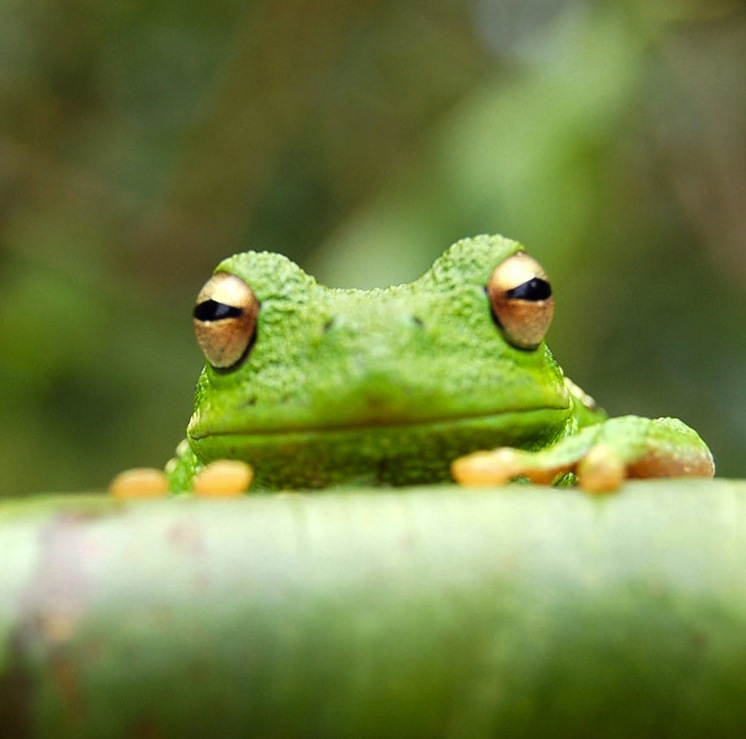
\includegraphics[width=0.5\textwidth]{frog.jpg}
\caption{\label{fig:frog}This is a figure caption.}
\end{figure}

\begin{table}
\centering
\begin{tabular}{l|r}
Item & Quantity \\\hline
Widgets & 42 \\
Gadgets & 13
\end{tabular}
\caption{\label{tab:widgets}An example table.}
\end{table}

\subsection{Mathematics}

\LaTeX{} is great at typesetting mathematics. Let $X_1, X_2, \ldots, X_n$ be a sequence of independent and identically distributed random variables with $\text{E}[X_i] = \mu$ and $\text{Var}[X_i] = \sigma^2 < \infty$, and let
$$S_n = \frac{X_1 + X_2 + \cdots + X_n}{n}
      = \frac{1}{n}\sum_{i}^{n} X_i$$
denote their mean. Then as $n$ approaches infinity, the random variables $\sqrt{n}(S_n - \mu)$ converge in distribution to a normal $\mathcal{N}(0, \sigma^2)$.

\subsection{Lists}

You can make lists with automatic numbering \dots

\begin{enumerate}
\item Like this,
\item and like this.
\end{enumerate}
\dots or bullet points \dots
\begin{itemize}
\item Like this,
\item and like this.
\end{itemize}

We hope you find write\LaTeX\ useful, and please let us know if you have any feedback using the help menu above.

\end{document}